% Created 2021-08-09 lun. 11:53
% Intended LaTeX compiler: pdflatex
\documentclass[11pt]{article}
\usepackage[utf8]{inputenc}
\usepackage[T1]{fontenc}
\usepackage{graphicx}
\usepackage{grffile}
\usepackage{longtable}
\usepackage{wrapfig}
\usepackage{rotating}
\usepackage[normalem]{ulem}
\usepackage{amsmath}
\usepackage{textcomp}
\usepackage{amssymb}
\usepackage{capt-of}
\usepackage{hyperref}
\author{Oumaima Hajji}
\date{\today}
\title{rapport stage}
\hypersetup{
 pdfauthor={Oumaima Hajji},
 pdftitle={rapport stage},
 pdfkeywords={},
 pdfsubject={},
 pdfcreator={Emacs 27.2 (Org mode 9.4.4)}, 
 pdflang={English}}
\begin{document}

\maketitle
\tableofcontents



\section{Abstract (TO EDIT - 0.5 pages)}
\label{sec:org3c07799}
As time goes on and the sciences progress exponentially, we find
ourselves in a position where it's hard for a scientist to fully
develop their research and present it for the others in a way that's
easy to grasp and reproduce. With the abundant number of research
papers written with no data attached to test them with, or the the
ones lost with no way to restore, it's time for the researchers to
change their attitude and work towards a more reproducible
approach. This is the main goal of the mooc which aims to teach all
the many ways a researcher can make every step of their process as
reproducible as possible. And so, in this project, our main aim was to
take care of making science more open and have it stored in an eternal
archiving space. This is the reason we worked to create a backend for
git-annex to handle the versioning of huge files during the entire
research process, and then allow the user to archive their findings on
Zenodo, and cite their results using the doi given by Zenodo. Not only
this, but we added other tools to the arsenal for the user to keep on
evolving their work and for them to restore their files whenever and
whereever they want with the use of our programs.  

\section{Introduction (TO EDIT - 1.5 pages)}
\label{sec:orge009df4}
En France, dans les dernières années, il y a un mouvement autour de la
science ouverte qui cherche à rendre toutes les publications et les
données de la recherche disponibles pour toute personne intéressée. Il
vise la dissolution des frontières strictes financées qui rendent des
articles de recherche importants prisonniers et limitent leur rayon
d'exposition. Son objectif est ainsi important puisque laisser ces
travaux indisponibles réduit les efforts de la recherche et complexifie
les recherches futures des autres scientifiques. Non seulement cela,
mais il limite aussi le taux de réutilisation du matériel et donc
cause l'augmentation du temps perdu pour atteindre un même résultat.

C'est là où parvient le plan national de la science ouverte qui oblige
les scientifiques à rendre ouvert l'accès pour leurs recherches
financées et leurs projets scientifiques. Il met en place un comité
qui gère tous ces efforts de structuration et qui planifie des points
de gestion de ce sujet. Afin d'atteindre ce but de la science ouverte,
le comité s'appuie sur les quatre principes de \emph{FAIR data} qui sont: 
\begin{description}
\item[{F: Faciles à retrouver}] Les données FAIR doivent être faciles à retrouver par l'humain et la
machine et donc il faut qu'elles aient des identificateurs uniques,
des descripteurs bien détaillés, et des métadonnées riches.

\item[{A: Accessibles}] Les données FAIR doivent être disponibles pour les communautés
auxquelles elles sont ouvertes. Elles doivent être récupérables
facilement avec l'utilisation de leur identificateur unique et leurs
métadonnées doivent aussi être disponibles.
Il y a des conditions qui surveillent la disponibilité de ces
données telles que les autorisations et les licences.

\item[{I: Interopérables}] Les données FAIR doivent respecter les règlements internationaux et
avoir des métadonnées qui sont précises et qui utilisent un
language clair et informatique international.

\item[{R: Réutilisables}] Les données FAIR doivent être réutilisables par d'autres personnes
et donc il faut qu'elles soient bien décrites et détaillées et que
les résultats soient vérifiables.
\end{description}

Maintenant que l'on connaît les quatre principes qui doivent être
respectés par toutes les données et que l'on comprend leur utilité,
on se pose une question logique au final: comment faire pour réussir
cet objectif? C'est là où se manifeste l'importance du mooc (Massive
open online course) qui cherche à éduquer les scientifiques à répondre
au maximum de ces contraintes. En effet, dans la première version du
mooc, l'objectif est d'expliquer comment bien prendre des notes et
rédiger un document computationnel qui peut être lu et compris par une
autre personne, et où on peut retracer le même acheminement logique de
l'expérience. Donc ce premier mooc touche déjà à des points du dernier principe de
la réutilisabilité des données. Pour ce qui concerne les autres
principes, le prochain mooc prioritise les autres principes puisqu'il
vise à faciliter le stockage et l'archivage des données pour les
rendre accessibles, retrouvables, et citables. C'est ainsi que l'on
entame le projet du stage qui aborde ce sujet de l'archivage pour
répondre au maximum des exigences des sciences ouvertes et pour
faciliter les tâches des scientifiques en leur fournissant tous les
outils dont ils ont besoin pour réussir ce but. 

\section{Etat de l'art (TO EDIT - 2.5 pages)}
\label{sec:orgbd601c3}
\subsection{Historique, gros fichiers (TO EDIT)}
\label{sec:orgb46a2de}
Dans la science moderne, particulièrement la science computationnelle
et la data science, on gère un énorme volume des fichiers et des
données qui évoluent fréquemment au cours du temps. Il faut donc
garder une trace de chaque version de données utilisées et du code
exécuté à un instant pour pouvoir garder une empreinte continue du
développement de la recherche et donc pour comprendre et suivre tous
les pas de l'expérience. C’est là où se manifeste l’importance de
‘Data Version Control’ dans un domaine de recherche où on manipule un
tas de données; on perd la reproductibilité du résultat quand on ne
manage pas du contrôle de données. C’est avec cette philosophie en
tête que l’on cherche à utiliser un outil pour s’occuper de cette
tâche.

Le logiciel que l’on a décidé d’utiliser est Git puisque c’est
l’outil le plus utilisé pour la gestion des versions. Mais il y a
toujours un problème avec cet outil malgré son excellente performance:
il ne permet pas de gérer les fichiers binaires de grande
taille. Cela est dû au fait qu’un dépôt Git stock toutes les versions
de chacun des fichiers ajoutés dedans. Ainsi, au fur et à mesure qu’un
projet avance, l’utilisateur se rend compte de l’inflation de la
taille de ce projet et donc les opérations importantes que l’on peut
effectuer comme fetch/pull ne seront plus performants. Il faut
aussi ne jamais dépasser 10 GB pour chaque dépôt car c’est la taille
maximale possible. Heureusement, Git a plusieurs extensions dont on
peut se servir quand on a des fichiers de grande taille. Les deux
outils les plus recommandés sont: git-annex et Git LFS.

\textbf{Git LFS} est une extension de Git qui permet de manipuler les fichiers
de grande taille en réduisant l'impact qu'ils ont sur le dépôt. Cela
est fait grâce à son mécanisme de téléchargement de versions
pertinentes. Mais ce processus engendre des problèmes de taille pour des
utilisateurs puisque les fichiers sont stockés 2 fois dans
leur intégralité (en local et dans le dépôt externe Github par
exemple), et donc cela veut dire que l'on perd de l'espace inutilement
parfois.
Un deuxième problème s'avère quand on veut supprimer un
unique blob dans un dépôt géré par Git LFS, puisqu'il y n'y a pas une
action directe à faire pour réussir cet objectif et libérer la place
de ce fichier dans le dépôt. Un utilisateur doit donc supprimer tout
son projet et recréer un deuxième projet avec les fichiers qu'il veut
inclure. Mais ce n'est pas une solution productive.

\textbf{git-annex} est un système de gestion et de partage des fichiers de
grande taille qui permet de les manager sans devoir enregistrer leur
contenu sur Git. Il utilise des liens symboliques qui pointent sur les
fichiers et stocke seulement les métadonnées de ces fichiers. C'est
grâce à ce mécanisme que l'on peut facilement gérer ses données en
choisissant à tout moment où les stocker (en local ou dans un dépôt
externe) en ne perdant pas de l'espace inutilement.
Il est donc plus intéressant pour nous car il répond à nos exigences
et il donne accès à plusieurs mécanismes de stockage en externe qui
vont être intéressants pour nous.

\subsection{Archivage}
\label{sec:org6c7732a}
Maintenant que l'on sait comment gérer les fichiers il faut passer à
l'autre étape importante dans ce procès qui est l'étape de
l'archivage. Dans le cadre de la recherche, c’est impératif de bien
archiver pas seulement ses trouvailles, mais aussi tous les outils
utilisés pour y arriver (Il faut mettre en disposition le code source,
les données utilisées, les notes détaillant les pistes prises, …). On
ne peut pas faire un puzzle sans avoir toutes les pièces
nécessaires.

Ainsi, quand un rechercheur archive bien ses travaux, il
garantit leur pérennité et assure leur disponibilité pour une
communauté. Non seulement cela, mais il peut aussi récupérer un
identificateur pérenne pour référencer ses travaux. Il existe
plusieurs outils à utiliser pour bien archiver les fruits de son
labeur, en particulier: Zenodo, Nakala, et figshare. Les trois sont
utilisés dans le domaine de la recherche et permettent de stocker,
partager, et préserver les travaux scientifiques. Ils fournissent
aussi un identificateur unique pour les bien citer et référencier.  Et
puisque les trois outils offrent des services similaires, on a décidé
de se servir de Zenodo qui est un outil multidisciplinaire (on peut
déposer des papiers de recherche, des datasets, des logiciels, des
rapports, \ldots{}) développé par OpenAIRE ( ) et exploité par CERN ( ).
C’est l’un des entrepôts les plus utilisés dans tous les domaines de
recherche qui ne coûte rien et qui permet d’avoir des dépôts de 50 GB
(\url{https://public.tableau.com/app/profile/bibdesponts/viz/tableauDATAv2\_0/Tableaudebord1}).


Maintenant que l’on connaît les deux parties importantes pour bien
gérer les gros fichiers et les archiver, il faut forger une liaison
directe entre elles. Un souci que l’on rencontre c’est que l’archivage
est une opération manuelle qui se fait sur les plateformes d’archivage
sans passer par un mécanisme d’automatisation. C’est donc parfois
compliqué de bien gérer les versions de ses fichiers en local avant de
les déplacer vers un entrepôt d’archivage. Une solution possible est
d’utiliser des raccourcis entre Zenodo et un serveur de Git. En effet,
il y a un raccourci entre Zenodo et github où les deux comptes de
l'utilisateur sont connectés pour lui permettre de mettre ses projets
github directement sur Zenodo et de les archiver facilement. Même si
ce mécanisme est facile à utiliser et garantit une automatisation du
processus, il y a toujours le problème de la taille des dépôts qui
sont hébergés sur Github. Un autre problème c’est le fait que ce
raccourci est personnalisé pour Github, et donc on ne peut pas faire
cela avec d'autres plateformes comme gitlab sans passer par des
bibliothèques ( link). Et même quand utilise une bibliothèque pour
faire ce lien Zenodo-Gitlab, il y a toujours un problème puisque cette
méthode permet juste de publier des fichiers sur Zenodo en utilisant
l'API et ne permet pas de faire plus que ça (on ne peut pas par
exemple récupérer des fichiers dans l’autre sens).


La proposition que j’ai est donc de commencer par git (sans passer par
ses serveurs) et de construire un chemin vers Zenodo. C’est ce que
l’on va faire git-annex en s’appuyant sur le mécanisme des remotes. Un
special remote de git-annex c’est un backend que l’on peut utiliser
pour transférer les données. Les commandes git-annex permettent de
contrôler le déplacement de ces données et de savoir où elles sont à
chaque moment. Il y a déjà une dizaine de remotes qui sont développés
par git-annex et sont prêts pour être configurés et utilisés (ex: adb,
Amazon S3, git lfs, …) , mais Zenodo ne figure pas dans cette
liste. On va donc implémenter un special remote git-annex pour Zenodo
qui va répondre à toutes nos attentes.

\section{Contributions (TO EDIT - 8 pages)}
\label{sec:orga7956f6}
\subsection{Modèle de données}
\label{sec:org70fd794}
Avant de commencer l’implémentation du remote, il y avait quelques
choix à faire pour savoir comment bien répondre à des problèmes qui
couvrent le côté git-annex mais aussi l’architecture et le modèle d’un
dépôt Zenodo.

La première question que l’on s’est posé c’était par rapport aux
contraintes sur les tailles et le nombre de fichiers. Puisque l’on a
déjà une information sur la taille maximale de tout le dépôt (50 GB
mais un utilisateur peut demander d’en avoir plus dans des cas
particuliers), il fallait aussi savoir si Zenodo impose des limites
sur le nombre des fichiers dans un dépôt. On a contacté Zenodo pour
poser cette question, et en attendant la réponse, on a aussi fait des
tests où on a déposé des milliers de fichiers de différentes
tailles. La réponse était positive et c'est donc possible de stocker
un nombre indéfini de fichiers mais la taille du dépôt ne doit pas
atteindre 50GB. C'est la seule limite imposée par Zenodo.


Le deuxième problème s’est avéré lors de la conception du remote; Il
fallait faire un choix de mappage remote git-annex / dépôt Zenodo. Les
deux entités sont différentes et alors le fonctionnement final de
notre mécanisme de gestion et d’archivage de données dépend de comment
on décide de relier les deux concepts. Un dépôt sur Zenodo c’est un
récipient où on peut mettre des fichiers de différents types et que
l’on peut publier à la fin pour archiver les fichiers. De l’autre
côté, un remote git-annex est un dépôt distant qu’il faut initialiser
et configurer afin de l’utiliser pour gérer les données. On peut donc
initialiser plusieurs remotes dans un répertoire de fichiers et on
peut choisir les fichiers à stocker dans un remote, et ceux à laisser
en local. Donc pour faire le mapping git-annex / Zenodo, on avait deux
possibilités: avoir une implémentation bijective 1-to-1 où on associe
chaque dépôt Zenodo à un remote git-annex, ou une relation surjective
où l’utilisateur choisit le nombre de dépôts Zenodo à lier à un seul
remote. La première option paraît la plus logique puisqu’elle permet
d’éviter les problèmes de confusion entre les dépôts Zenodo qui
peuvent d’avérer. L’utilisateur peut également créer un autre dépôt
Zenodo avec un nouveau remote git-annex s’il le souhaite; c'est
toujours possible d'initialiser plusieurs remotes git-annex dans la
même directory.


Le troisième problème est purement architectural; Zenodo a une
architecture plate et donc on n’a pas de notion de répertoire dans un
dépôt. Donc il fallait bien penser à comment structurer le dépôt pour
pouvoir retrouver facilement les fichiers que l’on met
dessus. Heureusement, et grâce à git-annex qui relie chaque fichier
annexé à une clé unique, on a pu trouver comment bien structurer le
dépôt Zenodo. Au lieu de laisser les noms des fichiers que l’on a en
local quand on fait un upload sur Zenodo, on a décidé de remplacer les
noms des fichiers par les clés. Et puisque l’on a un lien unique entre
le remote et le dépôt Zenodo, on peut facilement retrouver les
fichiers que l’on veut et les récupérer en local.

\subsection{Implémantation de remote Zenodo: le backend}
\label{sec:org86e4ec3}
\subsubsection{Introduction à l'API REST Zenodo}
\label{sec:org75316c8}
Afin de se communiquer avec Zenodo pour effectuer des
opérations sur les fichiers, il faut utiliser son API. La première
partie du processus est donc de comprendre comment elle fonctionne et de
la tester. On a fait les tests de manière chronologique en suivant le
tutorial mis en disposition par Zenodo (lien). On a donc créé une clé
qui permet d'authentifier l'utilisateur, et on a commencé par créer le
dépôt pour héberger les données et de les déposer dedans avec des
requêtes HTTP. On a aussi testé des autres opérations importantes
telles que la suppression des fichiers, la récupération d'un fichier
en utilisant son identifiant unique, la publication d'un dépôt, la
création des nouvelles versions d'un dépôt publié. En effet, les deux
dernières opérations sont très importantes pour nous puisque
l'archivage d'un fichier commence par sa publication (on obtient le
doi) et la création d'une nouvelle version d'un dépôt permet de
l'évoluer en gardant un identificateur pour chaque changement.
Au final, on a pu trouver un flow des requêtes API à lancer pour
pouvoir avoir un mécanisme logique qui permet un utilisateur de garder
une évolution gracieuse au cours de sa recherche:

\begin{figure}[htbp]
\centering
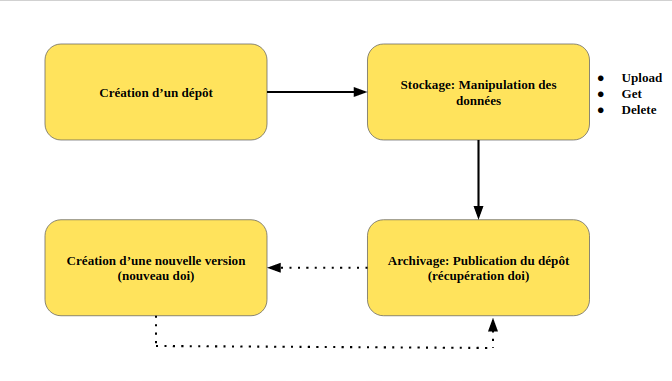
\includegraphics[width=.9\linewidth]{./flowchart.png}
\caption{\label{fig:orgaa2fcc4}flow chart}
\end{figure}

\subsubsection{AnnexRemote: la bibliothèque python utilisée}
\label{sec:org8c53dd8}
Maintenant que l'on peut facilement communiquer avec Zenodo et que
l'on a un blueprint de comment on veut structurer notre backend
Zenodo, il faut commencer son implémentation.

Afin d'implémenter un remote git-annex, il faut d'abord être sûr que
son programme implémente bien le protocole 'external special remote' de
git-annex qui fait le lien entre git-annex et un remote externe. En
effet, les deux bouts de la communication échangent des requêtes et des
réponses durant la période de l'exécution du programme, et donc pour
ne pas avoir des soucis de confusion des interactions, à chaque fois
l'une des deux parties prend l'initiative en n'envoyant que des
requêtes et l'autre partie répond alors avec des réponses à ces requêtes. 
C'est pour cette raison qu'il faut avoir un programme qui répond bien
à ces contraintes. On utilise donc la bibliothèque \textbf{AnnexRemote} de
python qui implémente la totalité du protocole et respecte toutes ses
spécifications. Il faut donc juste importer cette bibiliothèque dans
notre programme et définir une classe \emph{ZenodoRemote} qui extend la classe
\emph{SpecialRemote} (implémentée par \textbf{AnnexRemote}). Ensuite, on implémente
les fonctions de la classe avec les fonctionnalités qui sont uniques
à notre backend Zenodo. Toutes les fonctions de la création du dépôt,
suppression des fichiers, obtention d'un fichier, .. sont définies,
mais pour tout ce qui reste (par exemple, la création d'une nouvelle
version) c'est à nous d'ajouter.

\subsubsection{Les opérations principales du remote}
\label{sec:orgd98003f}
Chaque remote Zenodo doit être capable d'exécuter des opérations
principales qui servent à envoyer les fichiers sur le remote, les
manipuler, et les récupérer en local. Tout cela se fait avec les
fonctions du programme principal \textbf{git-annex-remote-zenodo}. Voici les
opérations essentielles implémentées dans le programme principal:

\begin{description}
\item[{Création du dépôt}] C'est la première étape du procès qui se fait une fois pour chaque
remote, on l'implémente donc lors de l'initialisation du remote
(dans la fonction \texttt{initremote} de la classe). On s'appuie sur la clé
donnée par l'utilisateur, ainsi que son choix Sandbox (FN) ou non,
pour envoyer une requête POST à l'API demandant la création du
dépôt. On récupère ensuite l'identifiant unique du dépôt ainsi que
d'autres informations (comme le lien à utiliser pour déposer les
fichiers), et on les stocke dans le fichier des configurations de
git-annex. On stocke aussi la clé unique de l'utilisateur pour ne
pas lui demander à chaque fois de la donner.

\item[{Envoi d'un fichier}] Cette opération peut s'exécuter plusieurs fois par l'utilisateur
lors de sa recherche, puisqu'elle permet de stocker les fichiers
dans un autre endroit où ils sont disponibles à tout moment pour
être observés ou récupérés. On implémente cette fonctionnalité dans
la fonction \texttt{transfer\_store} de la classe.
Pour commencer l'envoi des fichiers, il ne faut d'abord le lien vers
le dépôt que l'on récupère facilement avec la fonction \texttt{getconfig} de
l'annex. Après, on exploite le fait que git-annex donne à chaque
fichier annexé un identificateur unique (une clé SHA1), et on
utilise donc cet identificateur comme nom quand on dépose un fichier
sur Zenodo.

Ce choix d'implémentation nous permet de garder un lien
direct entre git-annex et Zenodo sans devoir passer par autres
étapes supplémentaires d'identification. On sait qu'un fichier File1
qui a un identificateur Key1 et qui est annexé en local est le même
que le fichier Key1 qui est dans le remote. Et puisque git-annex
s'appuie principalement sur les identificateurs des fichiers pour
les manipuler, maintenant, quand veut chercher un fichier dans le
remote, on peut faire ça directement sans devoir chercher le fichier
qui est relié à cet identificateur.

\item[{Récupération d'un fichier}] Afin de récupérer un fichier qui sur Zenodo en local, on peut
simplement faire une requête GET de l'API pour récupérer la liste
des fichiers qui sont dans le dépôt. Après, on peut chercher le
fichier dont le nom correspond à la clé git-annex que l'on veut
récupérer. Une fois trouvé, on peut récupérer l'identificateur
Zenodo donné à chaque fichier stocké dessus, et on utilise cet
identifiant pour télécharger ce fichier.

On ne peut pas directement télécharger un fichier sans connaître son
identificateur Zenodo unique. Cet identificateur est donné lors du
stockage du fichier sur Zenodo et est différent de l'identificateur
git-annex que l'on utilise pour renommer le fichier.

\item[{Vérification de l'existence d'un fichier}] Cette opération se fait plusieurs fois durant le procès puisqu'elle
est exécutée par git-annex à chaque fois que l'on cherche à savoir
l'état d'un fichier. Elle est donc lancée quand on
veut déposer un fichier (pour être sûr qu'il n'y est déjà pas),
quand on veut le récupérer, et quand on veut savoir où il est (la
commande 'git-annex whereis' par exemple).

En principe, on parcourt la liste des fichiers qui sont disponibles
sur le dépôt en comparant la clé git-annex donnée avec le nom du
fichier et on renvoie au final un booléen pour informer git-annex
de l'existence ou non de ce fichier dans le remote.

\item[{Suppression d'un fichier}] Afin d'envoyer un fichier, on s'assure déjà qu'il est disponible sur
le remote (s'il n'est pas là, on ne fait rien, et on ne considère
pas ça comme erreur). On récupère donc la liste des fichiers
disponibles dans le dépôt et on envoie une requête DELETE à l'API
avec l'identifiant unique de ce fichier.
\end{description}

\subsubsection{Les tests effectués}
\label{sec:org9e17c43}
Après chaque opération effectuée, s'il y a eu des problèmes, on évoque
une exception RemoteError avec le souci rencontré. On s'appuie sur
les codes retournés dans les réponses de l'API pour savoir le status
de la requête. Pour chaque opération, un code définit un état unique
et donc on peut imprimer l'erreur dans les messages de debug pour
l'utilisateur. C'est grâce à ces messages que l'on peut donc savoir
la source du problème (si cela parvient juste de la requête ou si
c'est un problème interne à Zenodo).

Donc lors des tests de fonctionnement du backend, et grâce à
l'inclusion d'un mode debug, on a pu s'assurer de la correction des
opérations et de la cohérence entre git-annex et l'API Zenodo.
Il y a eu des tests élémentaires pour chaque partie du programme
pour gérer les petites tâches avant de passer aux tests complets où
on a effectué toutes les opérations possibles sur le remote.
Les traces qui informent le déroulement de ce procès peuvent être
observées dans le fichier \texttt{journal.org}  (add fn ) où j'ai rédigé toutes les
notes qui concernent ce projet et les tests effectués tout au long
du stage avec les résultats trouvés.

\subsection{Archivage}
\label{sec:orgb711879}
\subsubsection{Archivage direct des données}
\label{sec:org196cb3f}
Quand la première partie de la gestion des données finit, et on stocke
tous les fichiers qui nous intéressent dans le remote, il faut
maintenant passer à la deuxième partie de l'archivage qui se fait
indépendamment de la première, et où on finalise son dépôt avec toutes
les métadonnées nécessaires avant de le publier.
Dans notre programme d'archivage \texttt{git-annex-disableremote.py}, on a
décidé de diviser les principales étapes de l'archivage en trois
parties logiques: la publication du dépôt, la transformation des
fichiers en remote web, et finalement la suppression du remote en
local. Chacune de ces étapes joue un rôle intrinsèque et la succession
des trois est ce que garantit l'archivage de notre dépôt.

\begin{description}
\item[{La publication du dépôt}] Afin de publier un dépôt sur Zenodo, il faut d'abord donner des
informations sur ce dépôt. On donne ainsi le choix à l'utilisateur
de choisir la manière dont il veut fixer les métadonnées: soit il
donne le path d'un fichier zenodo.json qui contient déjà les
métadonnées, ou il les donne manuellement sur le terminal en
répondant aux questions posées par le programme, ou il les configure
directement sur Zenodo. On fait des tests après pour s'assurer
qu'elles sont bien données, et on passe à l'étape suivante de la 
publication. C'est maintenant que l'on utilise l'opération \emph{publish}
de l'API pour finaliser la publication.

\item[{La transformation de fichiers en un web remote}] Cette étape est implémentée pour ajouter les fichiers que l'on vient
de publier dans un deuxième remote avant de supprimer ce remote (On
veut que git-annex ait au moins deux copies de chacun des
fichiers). Si on ne passe pas par cette étape, l'utilisateur perdra le
lien direct git-annex <-> Zenodo pour ces fichiers.
C'est pour cette raison que l'on reprend la liste des fichiers
(leurs noms ainsi que la clé git-annex) et que l'on récupère les
liens de téléchargement de chacun des fichiers avant de les ajouter
à un remote web avec la commande 'git-annex addurl'.
Maintenant, et grâce à cela, tous les fichiers sont toujours
enregistrés comme des copies dans l'annex même après la suppression
du remote Zenodo.

\item[{La suppression du remote en local}] On s'appuie sur un fichier \texttt{remote.log} de git-annex pour récupérer le
nom du remote afin de le supprimer. Ce fichier est accessible depuis
la branche git-annex de Git et est utilisé pour stocker toutes les
informations concernant les remotes git-annex.
On peut retrouver le nom du remote (que l'on lui a donné lors de
l'initialisation) grâce à l'identificateur du dépôt Zenodo. Une fois
trouvé, on utilise la commande 'git remote remove' pour supprimer le
remote.
\end{description}

\subsubsection{Création d'une nouvelle version après l'archivage d'un dépôt}
\label{sec:orgfba2c1b}
Cette opération n'est pas possible que si on essaye de créer une
nouvelle version d'un dépôt déjà publié. C'est l'outil qui permet de
faire évoluer ses fichiers même après publication.
On peut donc créer une nouvelle version d'un dépôt quand on finit
toutes les étapes de publications simplement en initialisant un
nouveau remote et en donnant l'identificateur du dépôt que l'on veut
utiliser pour créer la nouvelle version.
L'option à utiliser est newversion=id et notre programme prend soin
de toutes les opérations possibles comme il aurait fait avec un
nouveau dépôt. 
\subsubsection{Stockage d'une archive de données dans un autre dépôt comme copie}
\label{sec:orge998835}
Il y a aussi une étape que l'on fait au début de l'opération de
l'archivage qui est la création d'une archive contenant les fichiers
et le stockage de cette archive sur un nouveau dépôt Zenodo. 
Cette opération se fait indépendamment de git-annex et permet ainsi
d'avoir une autre copie des données dans un dépôt accessible par
l'utilisateur seulement sur le site web de Zenodo.
L'utilité de cette opération est de permettre à l'utilisateur de
garder une copie qu'il peut récupérer quand il veut sans passer par
git-annex. Il y a des autres fichiers qui sont stockés dans ce dépôt
autre que l'archive: \texttt{git-annex-info.json} et \texttt{restore\_archive.py}. Le
premier fichier contient des informations sur les fichiers tels que
leurs liens de téléchargements, leurs identifiants, et leurs
noms. Tandis que le deuxième est un script python à lancer par
l'utilisateur pour restaurer les fichiers de l'archive. 

\subsection{Restauration d'une archive}
\label{sec:orgcc12d0d}
La restauration d'une archive se fait grâce au script \texttt{restore\_archive}
que l'utilisateur peut télécharger depuis le dépôt Zenodo avant de le
lancer. Comme options, il faut fournir la clé Zenodo, l'option de
restauration, et il faut aussi indiquer si c'est le site officiel
Zenodo qui est utilisé ou le sandbox.
Au début, le programme télécharge l'archive et le fichier
\texttt{git-annex-info.json} depuis le dépôt avant d'extraire son
contenu. Maintenant, on se trouve avec des liens symboliques cassés
(git-annex utilise des liens symboliques pour pointer à où les
fichiers sont stockés). Il faut donc restaurer le contenu des fichiers
maintenant. Les trois options possibles de restauration sont:

\begin{description}
\item[{L'option simpledownload}] On supprime les liens symboliques en les remplaçant par les fichiers
que l'on télécharge grâce aux liens stockés dans le fichier json. Au
final, l'utilisateur se retrouve avec ses fichiers qui sont
maintenant disponibles dans un dossier simple.

\item[{L'option rebuildannex}] Dans ce cas, au lieu de remplacer les liens symboliques par les
fichiers, on crée des dossiers dont les paths sont ceux où pointent
les liens symboliques. On peut récupérer les paths grâce au fichier
json où on a stocké les informations.
Au final, les liens qui étaient cassés sont maintenant fonctionnels
de nouveau et ils pointent vers des fichiers qui sont stockés ailleurs.

\item[{L'option usegitannex}] Cette option est pour un utilisateur qui compte repasser à git-annex
lors de la récupération des fichiers. L'idée est donc d'initialiser
un répertoire Git et git-annex où on ajoute tous les fichiers après
leur restauration (la restauration se fait de manière simple comme
en \textbf{simpledownload}). Une fois les fichiers ajoutés en annex, on les
ajoute aussi à un remote web pour garder une deuxième copie en
externe.
Puisque l'on initialise git-annex, les fichiers donc auront des
nouvelles clés git-annex.
\end{description}

Quand on finit la restauration des fichiers, le programme supprime
l'archive et les deux autres fichiers utilisés.
\section{Evaluation (TO EDIT - 0.75 page)}
\label{sec:orgfbe6060}
Après avoir fini l'implémentation du remote Zenodo et tous les autres
programmes complémentaires (scripts python pour la publication et pour
la restauration de l'archive), la dernière contribution effectuée
était la rédaction d'un tutoriel permettant de tester et comprendre la
totalité des fonctionnalités du remote. Le fichier \texttt{walkthrough.org}
(add fn: link) contient un tutorial détaillé avec des
explications pour chacune des fonctionnalités mentionnées en
haut. Commençant par une introduction au sujet, et après dans une
deuxième partie, l'utilisateur peut comprendre comment manipuler les
données en local avec git-annex et avec le remote Zenodo. Ensuite, il
passe à l'étape de l'archivage des données par publication, avant de
finir par initialiser une nouvelle version du dépôt ou par restaurer
les fichiers en local.

Et puisque ce projet fait partie du mooc 2, la dernière partie du
procès sera son intégration dans ce mooc pour permettre aux
rechercheurs de l'utiliser. Puisque le mooc est ouvert pour toute
personne travaillant sur un projet scientifique, surtout les projets
de data science, alors avoir un backend Zenodo déjà développé avec un
tutorial et une documentation déjà prête, va faciliter leurs tâches de
gestion de données et d'archivage.

L'implémentation de ce remote Zenodo m'a aussi permis de commencer à
travailler sur un autre backend git-annex pour Nakala. En effet,
puisque nakala était l'un des outils d'archivage concurrent dont on a
parlé au début et que l'on a considéré moins intéressant que Zenodo
quand on a fait le choix, alors même s'il était un choix possible, il
a cédé sa place pour Zenodo. Mais une fois que l'on a fini avec
l'implémentation du backend Zenodo, on a décidé d'avancer un peu sur
le backend Nakala pendant la dernière semaine du stage. 

\section{Méthodologie et compétences développées (TO EDIT - 3 pages)}
\label{sec:org4b7419d}
\subsection{Méthodologie}
\label{sec:org34e5a53}
\subsubsection{Documentation de l'ensemble du processus (TO EDIT - 0.75 pages)}
\label{sec:org0544898}
Puisque le sujet principal de ce stage est fortement relié à la
recherche reproductible, et que le mooc cherche à inclure des conseils
pour aider les rechercheurs à atteindre ce but, alors la première
étape pour moi était de comprendre comment rendre mon travail
compréhensible et reproductible. Grâce au mooc 1, j'ai appris comment
prendre des notes détaillées dans un fichier computationnel (j'ai
utilisé des fichiers en org mode pour exécuter des bouts de code avec
des commentaires en texte). Cela m'a permis d'avoir la majorité de ma
recherche dans un fichier complet (\texttt{journal.org}) dans un ordre
chronologique où chaque entrée est une journée de travail. Grâce à ça,
je peux revenir en arrière pour relire des notes que j'avais prises
il y a des semaines en réexécutant le code en parallèle aussi.

J'avais aussi lu la documentation des outils et suivi un tutoriel pour
chacun d'eux avant de commencer l'implémentation du remote. C'est la
lecture de la documentation en parallèle avec l'exécution des exemples
de test qui m'a permet de saisir leur fonctionnement et leur utilité.
Commençant par git-annex où un tutorial complet est disponible sur le
site (add fn: lien). J'avais appris dans ce tutorial comment
manipuler les fichiers en local avec git-annex avant de créer un
remote USB pour faire mes premiers tests avec un backend.

Pour Zenodo, c'était pareil puisque des premiers exemples de
manipulation de l'API sont donnés dans le tutorial (add fn: lien)
mais pour le reste j'ai juste suivi la même logique en testant des
fonctionnalités plus complexes.

Les notes initiales que j'avais prises sont valables dans un fichier
org (\texttt{notes.org} (add fn: link)) avec des explications de chacun des outils utilisés et des
commentaires sur le sujet de la recherche reproductible que j'avais
noté pendant des ateliers auxquels j'ai assisté au début du stage. 

\subsubsection{Gestion du projet (TODO - 1 page)}
\label{sec:org46a805f}
\begin{itemize}
\item reunions hebdomadaires, agile,
\item gantt chart, a posteriori, planification légère
\item identifier mes propositions personnelles (que ce soit des
trouvailles ou des directions à ne pas emprunter)
\end{itemize}
\subsection{Compétences développées (TO EDIT - 1 page)}
\label{sec:orgf2e7103}
Durant les trois mois du stage, j'ai pu me voir progresser
graduellement dans plusieurs aspects, techniques ou
personnelles. Puisque ce stage en laboratoire est mon introduction
formelle au monde de la recherche professionnelle, l'acquisition des
connaissances s'est fait en deux modes parallèles: un premier mode
théorique où la réflexion était le point dominant, et un deuxième de
la pratique et l'expérimentation. Acquérir des compétences grâce à ce
style de travail est donc évident.

L'un de mes aspects personnels qui s'est bénéficié de cette
méthode est ma capacité à prendre des responsabilités et des
initiatives. En effet, durant toute la deuxième partie du stage où il
fallait se concentrer sur l'implémentation du remote, après avoir
compris le fonctionnement des outils, il y avait à chaque fois des
choix d'implémentation à faire pour chacune des actions de
remote. Commençant par des choix simples concernant les outils choisis
pour faire les actions (ex: les bibliothèques les plus convenables),
il y avait aussi des décisions plus impactantes comme les options de
restauration des fichiers de l'archive, et les choix de publication
donnés à l'utilisateur quand il veut archiver ses données.

J'ai aussi développé ma capacité de bien documenter et rédiger les
solutions trouvées. Cela a été inclus naturellement durant le procès
puisque à chaque fois que je fais une décision d'implémentation, je
teste d'abord les fonctionnalités sur des petits exemples dans mon
journal, en expliquant la logique derrière chaque idée et en dessinant
un tableau compréhensible par tout montrant toutes les parties du
processus bien présentées et détaillées. 

\section{Conclusion (TO EDIT - 1.5 pages)}
\label{sec:org9722282}
Pour conclure, durant les trois mois du stage, j'ai pu bien apprendre
les principes de la science ouverte et l'importance de
rendre ses travaux pas seulement compréhensibles par les autres, mais
aussi reproductibles. Le fait de bien archiver les bonnes versions de
ses données et son code avec son papier final de recherche s'est avéré
bien utile et important pour faciliter les travaux des autres et pour
automatiser la vérification des résultats. D'un point de vue personnel,
j'ai appris comment bien rédiger mon journal de laboratoire pendant
les mois de recherche pour permettre aux autres de revisiter mes idées
dans un ordre logique et chronologique.

Et pour ce qui concerne la partie technique de la gestion de versions
et de l'archivage, j'ai pu implémenter un backend Zenodo où on peut
stocker ses données tout au long de la période de recherche, avec
l'intermédiaire de git-annex qui gère les versions et le déplacement
des fichiers. Grâce à ce backend Zenodo, on gère la pérennité de
l'archivage des données et on facilite la tâche de référencement pour
un rechercheur puisqu'il peut citer ses travaux en utilisant le
doi. On a aussi pu implémenter des autres fonctionnalités permettant à
l'utilisateur de faire évoluer ses données publiées en créant des
nouvelles versions de son dépôt. La restauration des données
indépendamment de git-annex s'est aussi automatisée grâce à un
programme qui gère la récupération d'une archive des données et de
restaurer les fichiers qui figurent dedans en laissant le choix de
restauration à l'utilisateur.

Vers la fin de la période du stage, pendant la dernière semaine,
j'avais aussi commencé l'implémentation d'un autre backend git-annex
pour Nakala. J'avais suivi la même philosophie avec ce remote en
commençant par des tests d'API, avant de faire des choix
d'implémentation en gardant en tête l'architecture d'un dépôt Nakala
et les notions qui en sont dépendantes. Au final, la majorité des
fonctions du remote Nakala ont été implémentées, et j'ai aussi faits
des tests pour chacune des fonctions indépendamment des autres, mais
des tests globaux n'ont pas été effectués.

L'utilisation de Datalad a aussi été planifiée pour aider à bien gérer
les données puisque Datalad a une notion de modules et submodules et
donc il peut être intéressant si on veut garder la hiérarchie des
dossiers. Et puisque Datalad donne accès à un backend figshare pour
archiver ses données, on a étudié le cas de figshare lors de
l'implémentation du remote Zenodo pour comparer les décisions qui ont
été prises par Datalad pour structurer les données. Au final, on a
décidé de prioritiser Zenodo comme remote de git-annex et on n'a donc
pas pu avancer sur les idées que l'on avait pour inclure Datalad dans
ce procès.

En fin de compte, l'archivage et la gestion des versions ne sont que
deux points minuscules dans le trajet vers une recherche plus
reproductible. C'est pour raison qu'il reste autres parties à gérer
pour bien combler la totalité de ce sujet. Donc, l'une des étapes qui
sont intéressantes est la gestion du workflow et l'automatisation des
tâches de compilation et d'exécution du code. Snakemake est l'outil
choisi pour atteindre ce but et donc il reste à chercher comment
intégrer des commandes git-annex dans un fichier Snakemake pourque le
workflow soit complet et la gestion des versions du code et des
données se fasse de manière complète.

\section{Bibliographie (TODO)}
\label{sec:orga5503d8}
\end{document}